\documentclass[12pt, oneside, a4paper, chapter=TITLE,section=TITLE]{abntex2}

\usepackage{abntex2-ifrj} % pacote com customizações da classe abntex2 para uso no IFRJ-CVR

%Carregando alguns pacotes extras
\usepackage{float}
\usepackage{scalefnt}
\usepackage{supertabular,booktabs}
\usepackage{multirow}
\usepackage{graphicx}
\usepackage{rotating}

% ---
% Informações de dados para CAPA e FOLHA DE ROSTO
% ---
\titulo{Totem de Autoatendimento para Restaurantes de Cidades Pequenas}
\tipotrabalho{Relatório Técnico para Engenharia de Software}
\autor{Alunos: Gabriel Muzel e Mateus Iuri \\ Profa. Dra. Suéllen Martinelli }

\local{Capão Bonito}
\data{\today}
\programa{Tecnologia em Sistemas Inteligentes}
% Preâmbulo
\preambulo{\imprimirtipotrabalho\, desenvolvido pelos alunos Gabriel Muzel e Mateus Iuri como parte dos critérios de avaliação da disciplina ministrada pela Profa. Dra. Suéllen Martinelli. O trabalho investiga a viabilidade de um totem de autoatendimento para restaurantes de cidades pequenas, com foco em reduzir filas e apoiar a inclusão digital.
}

% --------------------------------
\makeindex % compila o índice remissivo (opcional)
% --------------------------------

% --------------------------------
% Início do documento
% --------------------------------
\begin{document}

% Retira espaço extra obsoleto entre as frases.
\frenchspacing

% --------------------------------
% ELEMENTOS PRÉ-TEXTUAIS
% --------------------------------
\pretextual
% ---
\imprimircapa % Capa
\imprimirfolhaderosto % Folha de rosto
% ---

% ---
% lista de ilustrações
\pdfbookmark[0]{\listfigurename}{lof} \listoffigures*
\cleardoublepage
% ---

% ---
% lista de tabelas
\pdfbookmark[0]{\listtablename}{lot}\listoftables*
\cleardoublepage
% ---

% ---
% inserir lista de quadros
\pdfbookmark[0]{\listofquadrosname}{loq} \listofquadros*
\cleardoublepage
% ---

% ---
% inserir lista de abreviaturas e siglas (opcional)
\begin{siglas}
  \item[ABNT] Associação Brasileira de Normas Técnicas
  \item[CSV] \textit{Comma-Separated Values}
  \item[PO] Product Owner
  \item[SM] Scrum Master
  \item[TCLE] Termo de Consentimento Livre e Esclarecido
  \item[WIP] Work In Progress
\end{siglas}
% ---

% ---
% inserir lista de símbolos
% ---
\begin{simbolos}
  \item[$N$] Número de participantes da pesquisa
\end{simbolos}
% ---

% ---
% sumario
\pdfbookmark[0]{\contentsname}{toc}
\tableofcontents*
% ---

% --------------------------------
% ELEMENTOS TEXTUAIS
\textual
% --------------------------------

\chapter{Introdução}

A Engenharia de Software (ES) aplica abordagens sistemáticas ao desenvolvimento de software. Segundo \cite{sommerville2016engenharia}, a área surgiu para enfrentar a ``Crise do Software'' na década de 1960, quando projetos ultrapassavam prazos e orçamentos. A volatilidade dos requisitos levou ao surgimento dos Métodos Ágeis, formalizados pelo Manifesto Ágil em 2001, que priorizam entregas contínuas, colaboração com o cliente e adaptação a mudanças \cite{prikladnicki2014ageis}.

Este relatório documenta a primeira entrega do projeto ``Totem de Autoatendimento para Restaurantes de Cidades Pequenas'', desenvolvido na disciplina de Engenharia de Software da FATEC Capão Bonito por Gabriel Muzel e Mateus Iuri, sob orientação da Profa. Dra. Suéllen Martinelli. O escopo desta entrega compreende o referencial teórico, a pesquisa com clientes, a Matriz CSD, as Histórias de Usuário, o \textit{Product Backlog} e o \textit{Sprint Backlog} da Sprint 1.

\chapter{Características do Projeto}

O tema definido pelo grupo é o desenvolvimento de um totem de autoatendimento voltado a restaurantes de cidades pequenas. A proposta parte da observação de filas no caixa, demora no atendimento e erros na anotação de pedidos, problemas relatados por clientes em Capão Bonito e região.

A solução prevista é um totem com tela sensível ao toque que permita visualizar o cardápio, montar o pedido, personalizar itens, pagar de forma integrada e receber uma senha de retirada. A pesquisa inicial também apontou a inclusão digital de idosos como ponto crítico, o que levou à previsão de um modo de acessibilidade e de atendimento híbrido, com funcionário disponível para dar suporte.

\section{Problema e Objetivo}

\textbf{Problema:} em restaurantes de cidades pequenas, o atendimento presencial tradicional frequentemente gera filas, erros de anotação e espera insatisfatória. Ao mesmo tempo, a introdução de tecnologia de autoatendimento pode excluir clientes com pouca familiaridade digital.

\textbf{Objetivo geral:} avaliar a viabilidade de um totem de autoatendimento que reduza filas e melhore a experiência do cliente, sem abrir mão da acessibilidade e do suporte humano.

\begin{itemize}
    \item Identificar as principais dores relatadas por clientes de restaurantes.
    \item Mensurar a receptividade à tecnologia de autoatendimento na região.
    \item Levantar as funcionalidades mais desejadas pelo público.
    \item Documentar requisitos por meio de Histórias de Usuário e critérios de aceitação.
    \item Planejar a primeira Sprint com base em priorização e estimativa de esforço.
\end{itemize}

\section{Metodologia Utilizada: SCRUM}

O SCRUM é um método ágil de gerenciamento de projetos complexos, estruturado em três pilares \cite{schwaber2017scrum}:

\begin{itemize}
    \item \textbf{Papéis:} o \textit{Product Owner} (PO) maximiza o valor do produto; o \textit{Scrum Master} remove impedimentos; e o \textit{Time de Desenvolvimento} é auto-organizável e cross-funcional.
    \item \textbf{Artefatos:} o \textit{Product Backlog}, o \textit{Sprint Backlog} e o Incremento.
    \item \textbf{Eventos:} a \textit{Sprint}, o \textit{Sprint Planning}, as \textit{Daily Meetings}, a \textit{Sprint Review} e a Retrospectiva.
\end{itemize}

A Engenharia de Requisitos complementa o SCRUM ao documentar necessidades na forma de \textit{User Stories}, no padrão ``Como um [tipo de usuário], eu quero [funcionalidade] para que [benefício]''. Cada história recebe critérios de aceitação no formato ``Dado que [contexto], quando [ação], então [resultado esperado]'' \cite{wazlawick2019engenharia}.

\chapter{Entrega Parcial 1}

Esta seção documenta o planejamento da primeira Sprint, realizado na Sprint Zero. A Sprint Zero consistiu na definição do tema, na escolha da técnica de coleta e na elaboração do instrumento de pesquisa.

\section{Planejamento da Pesquisa}

\textbf{Objetivo da Coleta:} compreender a viabilidade de um totem de autoatendimento em cidades pequenas, identificando as dores de clientes de restaurantes (filas, erros de pedidos) e a receptividade à tecnologia.

\textbf{Técnica Escolhida:}
\begin{enumerate}
    \item \textit{Questionário Online (Survey):} aplicado a clientes para mensurar a aceitação da tecnologia e levantar requisitos.
    \item \textit{Pesquisa Qualitativa (Pergunta Aberta):} para captar percepções subjetivas e preocupações sobre a implementação do totem.
\end{enumerate}

\textbf{Estratégia de Recrutamento:} divulgação do link do Google Forms em redes sociais (WhatsApp, Instagram) e grupos comunitários locais.

\textbf{Ética em Pesquisa:} foi disponibilizado um Termo de Consentimento Livre e Esclarecido (TCLE) no início do formulário. Todos os participantes consentiram voluntariamente em participar.

\textbf{Amostra:} 13 respostas anonimizadas, coletadas em 08 e 09 de setembro de 2026. A faixa etária predominante é de 18 a 35 anos (12 de 13).

\section{Termo de Consentimento Livre e Esclarecido (TCLE)}

\noindent\textbf{TERMO DE CONSENTIMENTO LIVRE E ESCLARECIDO}

Você está sendo convidado(a) a participar da pesquisa acadêmica \textbf{``Totem de Autoatendimento para Restaurantes de Cidades Pequenas''}, desenvolvida pelos alunos Gabriel Muzel e Mateus Iuri do curso de Tecnologia em Sistemas Inteligentes da FATEC Capão Bonito.

\textbf{Objetivo:} compreender as necessidades de clientes para o desenvolvimento de um protótipo de totem de autoatendimento. \\
\textbf{Procedimentos:} sua participação consiste em responder a um questionário online com duração de 3 a 5 minutos. \\
\textbf{Riscos e Benefícios:} os riscos são mínimos (cansaço ao responder). Os benefícios incluem contribuir para o desenvolvimento de uma solução tecnológica local. \\
\textbf{Confidencialidade:} suas respostas são anônimas. Nenhum dado pessoal (nome, telefone, e-mail) foi coletado. \\
\textbf{Voluntariedade:} você pode desistir de participar a qualquer momento sem prejuízo. Ao clicar em ``Sim'', você concorda com estes termos.

\section{Artefato de Coleta}

Abaixo está o resumo do instrumento de coleta aplicado aos clientes via Google Forms.

\noindent\textbf{QUESTIONÁRIO APLICADO}
\begin{enumerate}
    \item \textbf{Qual é a sua faixa etária?} (múltipla escolha)
    \item \textbf{Com que frequência você costuma frequentar restaurantes?} (múltipla escolha)
    \item \textbf{Como você avalia o tempo de espera para fazer o pedido e ser atendido?} (múltipla escolha)
    \item \textbf{Qual é a sua maior frustração ao fazer um pedido em um restaurante hoje?} (múltipla escolha)
    \item \textbf{Você já utilizou totens de autoatendimento em restaurantes?} (múltipla escolha)
    \item \textbf{Em uma cidade pequena, como você se sentiria em fazer seu pedido em um totem?} (múltipla escolha)
    \item \textbf{Quais funcionalidades você consideraria MAIS importantes?} (caixas de seleção)
    \item \textbf{Você acredita que um totem ajudaria a reduzir as filas?} (escala de Likert)
    \item \textbf{Deixe uma sugestão, ideia ou preocupação sobre o uso do totem.} (resposta aberta)
\end{enumerate}

\section{Dados Coletados, Anonimizados e Planilhados}

Os dados coletados foram tabulados de forma anônima. A Tabela~\ref{tab:dados_quantitativos} apresenta o resumo dos dados quantitativos.

\begin{table}[!ht]
\centering
\caption{Resumo dos Dados Quantitativos Coletados}
\resizebox{\textwidth}{!}{%
\begin{tabular}{@{}llp{7cm}@{}}
\toprule
\textbf{Categoria} & \textbf{Resposta} & \textbf{Resultado (N = 13)} \\ \midrule
\textbf{Faixa Etária} & 18 a 25 / 26 a 35 / 46 a 60 & 6 (46,2\%) / 6 (46,2\%) / 1 (7,7\%) \\
\textbf{Frequência} & 1 a 2 vezes/mês / 1 vez/semana / mais de 2x/semana / raramente & 6 (46,2\%) / 3 (23,1\%) / 2 (15,4\%) / 2 (15,4\%) \\
\textbf{Avaliação da Espera} & Regular / Bom / Excelente & 8 (61,5\%) / 4 (30,8\%) / 1 (7,7\%) \\
\textbf{Maior Frustração} & Filas no caixa / Dificuldade de ver cardápio / Demora do garçom / Erros na anotação & 4 (30,8\%) / 4 (30,8\%) / 3 (23,1\%) / 2 (15,4\%) \\
\textbf{Experiência com Totem} & Sim, gostei / Sim, com dificuldades / Nunca utilizei & 10 (76,9\%) / 2 (15,4\%) / 1 (7,7\%) \\
\textbf{Conforto com o Totem} & Muito confortável / Indiferente / Pouco confortável & 5 (38,5\%) / 7 (53,8\%) / 1 (7,7\%) \\
\textbf{Reduzir Filas?} & Concordo totalmente / Concordo parcialmente & 7 (53,8\%) / 6 (46,2\%) \\ \bottomrule
\end{tabular}%
}
\label{tab:dados_quantitativos}
\end{table}

\textbf{Análise Qualitativa (Pergunta Aberta):} das 13 respostas, 7 trouxeram comentários. A inclusão digital de idosos é a preocupação mais frequente: 5 participantes citaram pessoas mais velhas ou pouca familiaridade com tecnologia. As sugestões incluem design intuitivo, funcionário treinado e carismático para suporte e manutenção do atendimento humano. As funcionalidades mais marcadas foram pagamento integrado (10), personalização (9), emissão de senha (8), fotos (5), acessibilidade (5) e programa de fidelidade (5).

\section{Matriz CSD}

\begin{table}[!ht]
\centering
\caption{Matriz CSD do Projeto com base nos dados coletados}
\resizebox{\textwidth}{!}{%
\begin{tabular}{@{}p{5cm}p{5cm}p{5cm}@{}}
\toprule
\textbf{CERTEZAS} & \textbf{SUPOSIÇÕES} & \textbf{DÚVIDAS} \\ \midrule
O totem agiliza o pedido e reduz filas no caixa. & O totem aumentará o ticket médio de vendas (upselling). & Qual o custo real de hardware e software viável para a região? \\
Pagamento integrado, personalização e senha são as funções mais desejadas. & Clientes mais velhos precisarão de auxílio de um funcionário treinado. & Como será feita a manutenção técnica e a atualização do cardápio? \\
5 participantes citaram idosos ou pouca familiaridade com tecnologia. & O design deve ser altamente intuitivo e limpo. & O totem deve substituir totalmente o caixa ou apenas auxiliar? \\
A emissão de senha é essencial para o fluxo de retirada. & A internet local é estável o suficiente para transações. & Quais métodos de pagamento são realmente indispensáveis? \\ \bottomrule
\end{tabular}%
}
\label{tab:matriz_csd}
\end{table}

\section{User Stories}

Com base nos dados, foram elaboradas as seguintes Histórias de Usuário.

\begin{itemize}
    \item \textbf{US01: Visualizar Cardápio.} Como um cliente, eu quero visualizar o cardápio com fotos e descrições para que eu possa escolher meu pedido de forma atrativa. \\
    \textit{Critério de Aceitação:} Dado que o cliente acessa o totem, quando seleciona ``Cardápio'', então o sistema exibe os produtos divididos por categorias com preços e fotos.

    \item \textbf{US02: Adicionar Item e Quantidade.} Como um cliente, eu quero adicionar itens e definir a quantidade para que eu possa montar minha refeição completa. \\
    \textit{Critério de Aceitação:} Dado que o cliente está vendo um produto, quando clica em ``Adicionar'', então o item vai para o carrinho e permite aumentar a quantidade.

    \item \textbf{US03: Personalizar Pedido.} Como um cliente, eu quero escolher os ingredientes do meu lanche para que eu possa comer exatamente como gosto. \\
    \textit{Critério de Aceitação:} Dado que o item permite customização, quando o cliente acessa o item, então o sistema exibe opções para remover ingredientes (ex: sem cebola) ou adicionar extras (ex: bacon).

    \item \textbf{US04: Realizar Pagamento Integrado.} Como um cliente, eu quero pagar meu pedido no totem usando Cartão ou PIX para que eu não precise enfrentar a fila do caixa. \\
    \textit{Critério de Aceitação:} Dado que o carrinho está preenchido, quando o cliente seleciona ``Finalizar Pedido'', então o sistema oferece as opções de pagamento e processa a transação.

    \item \textbf{US05: Emitir Comprovante e Senha.} Como um cliente, eu quero receber uma senha após pagar para que eu possa retirar meu pedido no balcão. \\
    \textit{Critério de Aceitação:} Dado que o pagamento foi aprovado, quando a tela de sucesso é exibida, então o sistema mostra a senha numérica em destaque.

    \item \textbf{US06: Acessibilidade (Modo Fácil).} Como um cliente idoso, eu quero uma opção de tela com letras maiores e instruções visuais simples para que eu consiga fazer meu pedido sozinho. \\
    \textit{Critério de Aceitação:} Dado que a tela inicial é exibida, quando o usuário toca no botão de acessibilidade, então o sistema aumenta as fontes e simplifica os botões.

    \item \textbf{US07: Suporte ao Atendente (Chamar Ajuda).} Como um cliente com dificuldades, eu quero um botão para chamar o atendente para que ele me ajude a finalizar o pedido no totem. \\
    \textit{Critério de Aceitação:} Dado que o cliente está em qualquer tela, quando ele toca em ``Preciso de Ajuda'', então o sistema emite um alerta para o balcão/cozinha.
\end{itemize}

\section{Product Backlog}

\begin{table}[!ht]
\centering
\caption{Product Backlog do Totem de Autoatendimento}
\resizebox{\textwidth}{!}{%
\begin{tabular}{@{}clcp{5cm}p{4cm}@{}}
\toprule
\textbf{ID} & \textbf{Nome da Funcionalidade} & \textbf{Imp.} & \textbf{PH} & \textbf{Como Demonstrar} \\ \midrule
01 & Visualizar Cardápio com Fotos & 30 & 5 & Abrir o totem, ver a tela inicial e navegar entre as categorias \\
02 & Adicionar ao Carrinho & 30 & 3 & Selecionar um hambúrguer e adicionar 2 refrigerantes \\
03 & Personalização de Itens & 30 & 8 & Selecionar ``X-Burger'' e remover o tomate \\
04 & Pagamento Integrado (PIX/Cartão) & 30 & 13 & Finalizar pedido e simular pagamento via API \\
05 & Tela de Sucesso e Senha & 25 & 3 & Pagar e visualizar a tela de senha gerada \\
06 & Painel de Acompanhamento (Admin) & 30 & 8 & Acessar rota /admin e ver pedidos em tempo real \\
07 & Acessibilidade (Modo Fácil) & 25 & 5 & Ativar botão de alto contraste e aumentar fontes \\
08 & Botão de Ajuda / Suporte & 20 & 3 & Clicar em ``Ajuda'' e ver o alerta na cozinha \\
09 & Cadastro de Produtos (Admin) & 20 & 5 & Inserir um novo produto no banco de dados \\
10 & Edição/Exclusão de Produtos (Admin) & 15 & 3 & Alterar o preço de um item existente \\
11 & Relatório de Vendas Diárias (Admin) & 15 & 5 & Exportar lista de pedidos do dia em CSV \\
12 & Modo de Espera (Atração) & 5 & 2 & Tela rodando vídeos enquanto ninguém interage \\ \bottomrule
\end{tabular}%
}
\label{tab:product_backlog}
\end{table}

\section{Sprint Backlog}

\begin{sidewaystable}
\centering
\caption{Sprint Backlog: Sprint 1}
\resizebox{0.95\textheight}{!}{%
\begin{tabular}{@{}p{3cm}p{7.5cm}cp{2cm}@{}}
\toprule
\textbf{História} & \textbf{Tarefas Técnicas} & \textbf{Resp.} & \textbf{Status} \\ \midrule
\multirow{3}{3cm}{\raggedright US01: Visualizar Cardápio} & 1. Criar protótipo de alta fidelidade no Figma. & Gabriel & A Fazer \\
& 2. Criar estrutura HTML/CSS da tela de cardápio. & Mateus & Em Andamento \\
& 3. Integrar com API/JSON de produtos. & Mateus & A Fazer \\ \midrule
\multirow{3}{3cm}{\raggedright US02: Adicionar Item} & 1. Implementar estado global do carrinho (Context). & Gabriel & A Fazer \\
& 2. Criar componente botão ``Adicionar''. & Gabriel & A Fazer \\
& 3. Criar drawer lateral do carrinho. & Mateus & Para Verificar \\ \midrule
\multirow{3}{3cm}{\raggedright US03: Personalizar Pedido} & 1. Criar tela modal de opções de ingredientes. & Mateus & A Fazer \\
& 2. Desenvolver lógica de subtração/acréscimo de preços. & Gabriel & A Fazer \\
& 3. Testar fluxo de item personalizado. & Gabriel & A Fazer \\ \bottomrule
\end{tabular}%
}
\label{tab:sprint_backlog}
\end{sidewaystable}

% ---------------------------------
% ELEMENTOS PÓS-TEXTUAIS
% ---------------------------------
\phantompart
\postextual

% ---------------------------------
% Referências bibliográficas
% ---------------------------------
\bibliography{../documentos/references}

% ---------------------------------
% Glossário
% ---------------------------------

% ---------------------------------
% Apêndices
% ---------------------------------
\begin{apendicesenv}
\partapendices

\chapter{Termo de Consentimento Livre e Esclarecido}

\begin{figure}[!ht]
\setlength{\itemsep}{0pt}
\setlength{\parskip}{0pt}
\centering
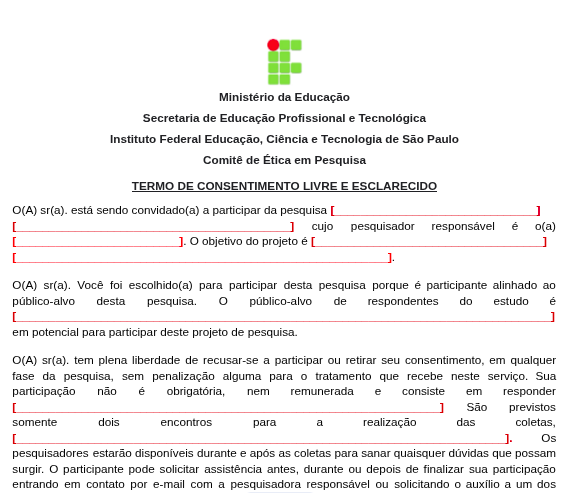
\includegraphics[width=0.7\columnwidth]{imagens/print_TCLE.png}
\caption{Formulário de consentimento apresentado no início da pesquisa.}
\end{figure}

\end{apendicesenv}

% ----------------------------------------------
% Anexos
% ----------------------------------------------
\begin{anexosenv}
\partanexos

\chapter{Questionário Aplicado}

O instrumento completo foi aplicado via Google Forms e continha nove perguntas, entre múltipla escolha, caixas de seleção, escala de Likert e resposta aberta. A Tabela~\ref{tab:dados_quantitativos} resume as respostas quantitativas.

\end{anexosenv}

%------------------------------------------------------
% INDICE REMISSIVO
%------------------------------------------------------
\phantompart
\printindex

\end{document}
